\subchapter{Goals}{Implement a live camera system and optimize its boot
time.}

Here's a description of the system that we are going to build and
optimize in terms of boot time:

Hardware:
\begin{itemize}
\item Main board: Beagle Bone Black (Regular or Wireless), with an ARM
Cortex A8 SoC (AM335x from Texas Instruments).
\item Extended by a 4 inch LCD cape
\item Connected to a USB webcam
\end{itemize}

Software:
\begin{itemize}
\item Bootloader: U-Boot
\item Operating system: Linux
\item User space: ffmpeg video player
\item Build system: Buildroot
\item Functionality: as soon as the system has booted, display
      the video from the USB webcam.
\end{itemize}

\begin{center}
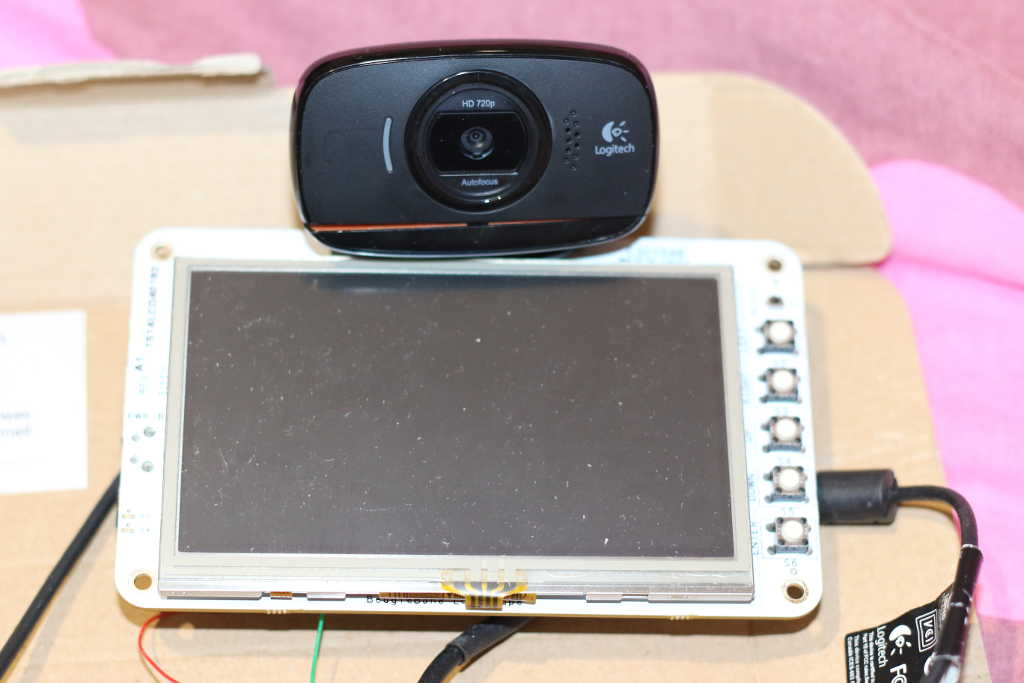
\includegraphics[width=8cm]{labs/boot-time-goals/goal.jpg}
\end{center}
